% Hình: Quy trình Seg-Grad-CAM và bản đồ nhiệt phủ chồng (Mục 3.7)
\documentclass[border=6pt]{standalone}
\usepackage[utf8]{vietnam}
\usepackage{amsmath,amssymb}
\usepackage{graphicx}
\usepackage{xcolor}
\usepackage{tikz}
\usetikzlibrary{positioning,fit,arrows.meta,calc,backgrounds}

\definecolor{qpurple}{HTML}{7E57C2}
\definecolor{qfill}{HTML}{ECE3F7}
\definecolor{cvblue}{HTML}{35618E}
\definecolor{cvbluefill}{HTML}{DCE7F2}
\definecolor{slate}{HTML}{5B6470}
\definecolor{slatefill}{HTML}{EDEFF2}
\definecolor{inkdark}{HTML}{23272E}

\tikzset{
  >={Stealth[length=2.4mm]},
  every node/.style={font=\sffamily\small, text=inkdark},
  proc/.style={draw=cvblue, fill=cvbluefill, rounded corners=2pt, thick, align=center, minimum height=10mm, minimum width=22mm},
  math/.style={draw=qpurple, fill=qfill, rounded corners=2pt, thick, align=center, minimum height=10mm, minimum width=24mm},
  frame/.style={draw=slate, line width=0.8pt, inner sep=0pt},
  flow/.style={-{Stealth[length=2.4mm]}, line width=0.9pt, draw=inkdark},
  grad/.style={-{Stealth[length=2.2mm]}, line width=1pt, draw=qpurple, dashed}, 
  lbl/.style={font=\sffamily\scriptsize, text=slate},
}

\begin{document}
\begin{tikzpicture}
  % ==========================================
  % HÀNG 1: FORWARD PASS 
  % Nới rộng khoảng cách ngang (right=16mm đến 18mm)
  % ==========================================
  \node[frame] (img) {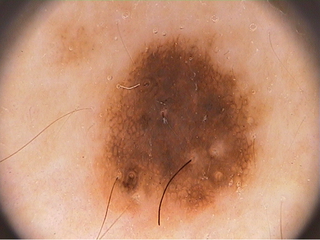
\includegraphics[width=2.5cm, height=2.5cm]{ph2_image.png}};
  \node[lbl, above=1.5mm of img] {Ảnh $X$};

  \node[proc, right=16mm of img] (net) {Kiến trúc mạng};
  \node[proc, right=16mm of net] (act) {Bản đồ kích hoạt\\ $A^k$};
  \node[math, right=18mm of act, fill=qfill!60] (score) {$S = \sum_{(i,j)\in\mathcal{R}} \hat{Y}_{i,j}$};

  \draw[flow] (img) -- (net);
  \draw[flow] (net) -- (act);
  
  % Chữ "Dự đoán Y" nay đã có không gian rộng rãi trên mũi tên
  \draw[flow] (act) -- (score) node[midway, above=1mm, lbl] {Dự đoán $\hat{Y}$};

  % ==========================================
  % HÀNG 2: BACKWARD PASS
  % Ép khoảng cách dọc 28mm tạo rãnh sâu, chống đè chữ
  % ==========================================
  \node[frame, below=28mm of img] (heat) {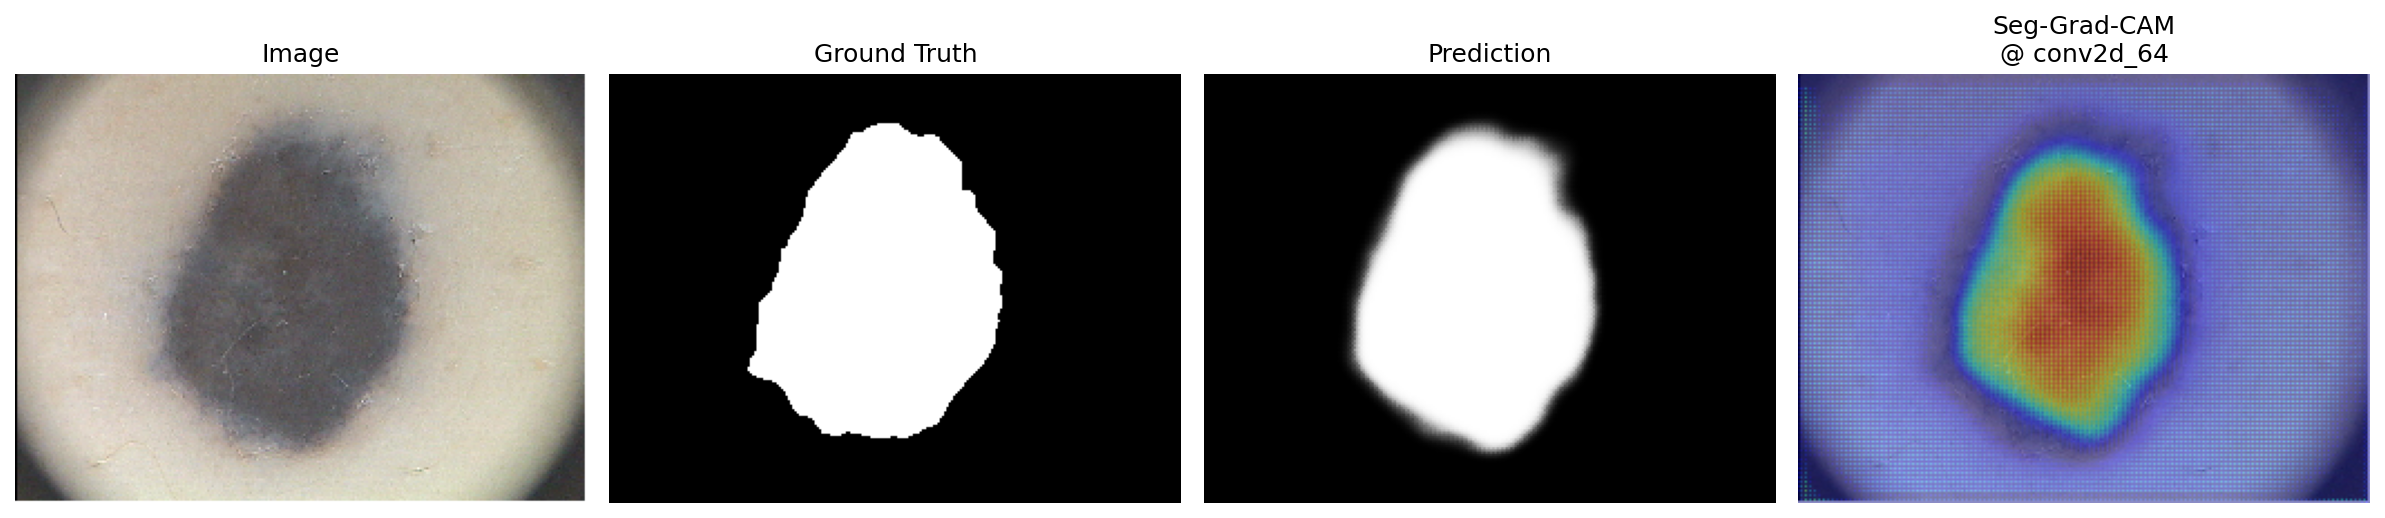
\includegraphics[width=2.5cm, height=2.5cm]{seggradcam_sample.png}};
  \node[lbl, above=1.5mm of heat] {Seg-Grad-CAM};

  \node[math, below=28mm of net] (cam) {$\mathrm{ReLU}\!\Big(\sum_k \alpha_k A^k\Big)$};
  \node[math, below=28mm of score] (alpha) {$\alpha_k=\dfrac{1}{Z}\sum_{i,j}\dfrac{\partial S}{\partial A^k_{i,j}}$};

  % ==========================================
  % KẾT NỐI HÀNG 2 VÀ CÁC ĐƯỜNG CHÉO
  % ==========================================
  \draw[grad] (score) -- (alpha) node[midway, right=1mm, lbl] {Lan truyền ngược};
  \draw[flow] (act.south) -- (alpha.north west) node[midway, sloped, above=1mm, lbl] {Đặc trưng};
  \draw[flow] (act.south) -- (cam.north east) node[midway, sloped, above=1mm, lbl] {$A^k$};
  \draw[flow] (alpha) -- (cam) node[midway, above=1mm, lbl] {Trọng số $\alpha_k$};
  \draw[flow] (cam) -- (heat);

  % ==========================================
  % THANH MÀU (COLORBAR)
  % ==========================================
  \begin{scope}[shift={($(heat.south west)+(0,-8mm)$)}]
    \shade[left color=cvblue, right color=red] (0,0) rectangle (2.5, 0.25);
    \draw[slate, line width=0.6pt] (0,0) rectangle (2.5, 0.25);
    \node[lbl, right=1mm] at (2.5, 0.125) {Cao};
    \node[lbl, left=1mm] at (0, 0.125) {Thấp};
  \end{scope}

\end{tikzpicture}
\end{document}